\graphicspath{ {./figures/} }
\section{Research}
\subsection{Basic Dynamics in Quadrupeds}
\subsection{Kinematics}
 Kinematics is  often referred to as the geometry of motion and describes the motion of points, bodies and systems of bodies without considering the forces that describe the motion. A kinematics problem begins by describing the geometry of the system and declaring the initial conditions of any known values of position, velocity and/or acceleration of points within the system. Then, using arguments from geometry, the position, velocity and acceleration of any unknown parts of the system can be determined. Using kinematics there are a variety of different calculations that can be done to help create an accurate and useful model of a robot. 
    \subsubsection{Forward Kinematics}
    Forward Kinematics refers to the use of kinematic equations to determine the position, usually in x, y, z coordinate space, of an end effector given specific joint parameters with relation to a specific reference point. In the case of a serial manipulator, this is very useful in understanding where the end of the robot will be if given a set of joint values. There are many different ways of calculating forward kinematics, however one of the most universally accepted and used methods is through the use of Denavit–Hartenberg parameters (DH parameters).
    \subsubsection{DH Parameters}
    In mechanical engineering and robotics, DH parameters are the four parameters associated with a particular convention for attaching reference frames to the links of a spatial kinematic chain, or serial robot manipulator.
    \begin{center}
    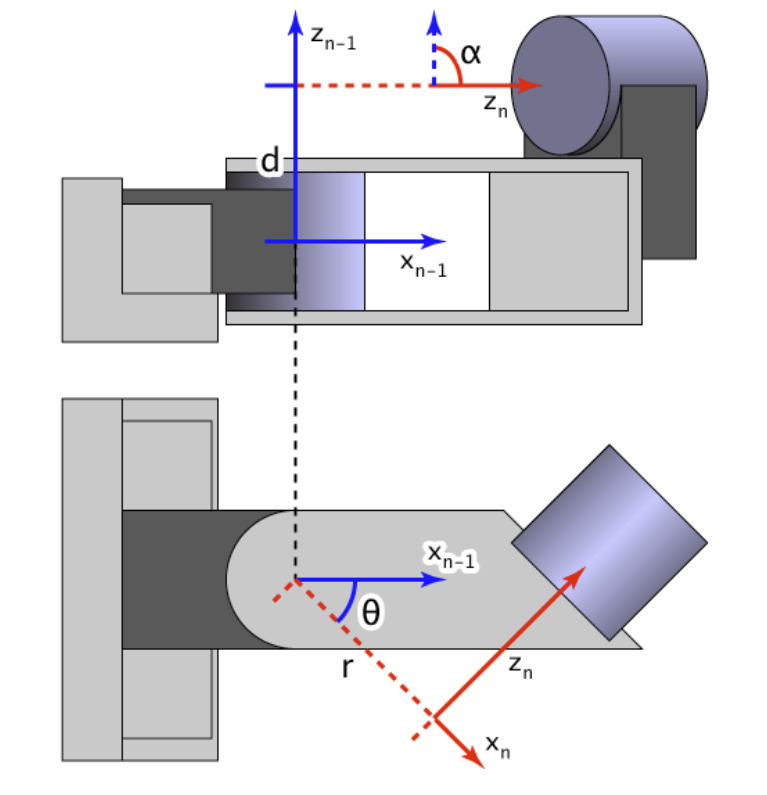
\includegraphics[width=75mm]{Dh.PNG}
    \end{center}
    Coordinate frames are attached to the joints between two links such that one transformation is associated with the joint, [Z], and the second is associated with the link [X]. The coordinate transformations along a serial robot consisting of n links form the kinematics equations of the robot. At its core D-H parameters are coordinate frames attached to the joints between two links such that one transformation is associated with the joint denoted as Z, and the other is associated with the link denoted as X. By multiplying these together you can describe a single link and its joint in a robot manipulator. The coordinate transformations along an entire serial robot consisting of n links form the kinematics equations of the robot.
    \begin{equation}
    [T] = [Z_1][X_1][Z_2][X_2]...[X_n[]_z-_1][Z_n][X_n]
    \end{equation}
    The coordinate transformations [Z] and [X], are determined by modeling the joints connecting the links as either hinged or sliding joints. By doing this, each of the joints can then be further described by a unique line S in space that forms the joint axis and define the relative movement of the two links. A typical serial robot is characterized by a sequence of these lines. For example in a six degree of freedom serial manipulator there are six Si where i = 1,...,6, one for each joint in the robot. For each sequence of lines Si and Si+1, there is a common normal line Ai,i+1. The system of six joint axes Si and five common normal lines Ai,i+1 form the kinematic skeleton of this six degree of freedom serial robot. Denavit and Hartenberg introduced the convention that Z 

\subsection{Gaits}
    \subsubsection{What is a gait}
    A gait is the motion of taking  a step. This includes the motion of each joint, the time at each place, the speed of motion and the time between cycles. In the case of a quadruped robot, the 
    
    \subsubsection{Types of gaits}
    




